\documentclass[11pt]{amsart}
\usepackage{amsmath,amsthm,amssymb,amsfonts,epic,epsfig,latexsym,enumerate}
\usepackage{enumitem}
\usepackage[titlenotnumbered,linesnumbered,noend,plain]{algorithm2e}
\usepackage{listings}
\usepackage{fullpage}

\newtheorem{lemma}{Lemma}
\usepackage{url}

\SetKwProg{Fn}{}{}{}

\parindent 0cm
\thispagestyle{empty}

\begin{document}



%\thispagestyle{empty}

%\hspace{0.11cm} \vspace{2cm}

\title{
Com S 311 Spring 2021\\
Exam 2
}

\maketitle


\vspace{-.8cm}
\begin{center}
{\bf Due:  April 22 7:59 p.m.}

\smallskip
\textbf{You must turn in a single pdf with your typed answers by 7:59 p.m.}\\
\textbf{\\Haadi Majeed}\\
\end{center}

\medskip

\section*{Guidelines}


\begin{itemize}

\item %It is important to know whether you really know. 
For each problem, if you write  the statement ``I do not know how to solve this problem'' (and nothing else), you will receive 20\% credit for that problem. If you do write a solution, then your grade could be anywhere between 0\% to 100\%.
To receive this 20\% credit, you must explicitly state that you do not know how to solve the problem.

\item You are \textbf{not} allowed to discuss the problems with anyone. You are allowed to use the textbook and notes. Do \textbf{not} copy solutions from the internet. Your writing should demonstrate that you understand the proofs completely.

\item When proofs are required, you should make them both clear and rigorous. Do not hand-waive.

 \item Please submit your assignment on the given Canvas exam.
 \begin{itemize}
\item  You \textbf{must} type your solutions, except manual tree drawing. Please submit a PDF version.
\item Please make sure that the file you submit is not corrupted and that its size is reasonable (e.g., roughly at most 10-11 MB).
\begin{center}
\emph{If we cannot open your file, your exam will not be graded.}
\end{center}
\end{itemize}

\item Any concerns about grading should be expressed within one week of
returning the exam. 
 
\end{itemize}


\newpage
\hrulefill \\

\textbf{Problem 1:} (Minimum Spanning Trees)\hfill (20 Points)\\

(a) Construct a minimum spanning tree for the graph below on the left. Draw the tree by adding edges to the graph on the right.

\begin{figure}[htb]
\begin{center}
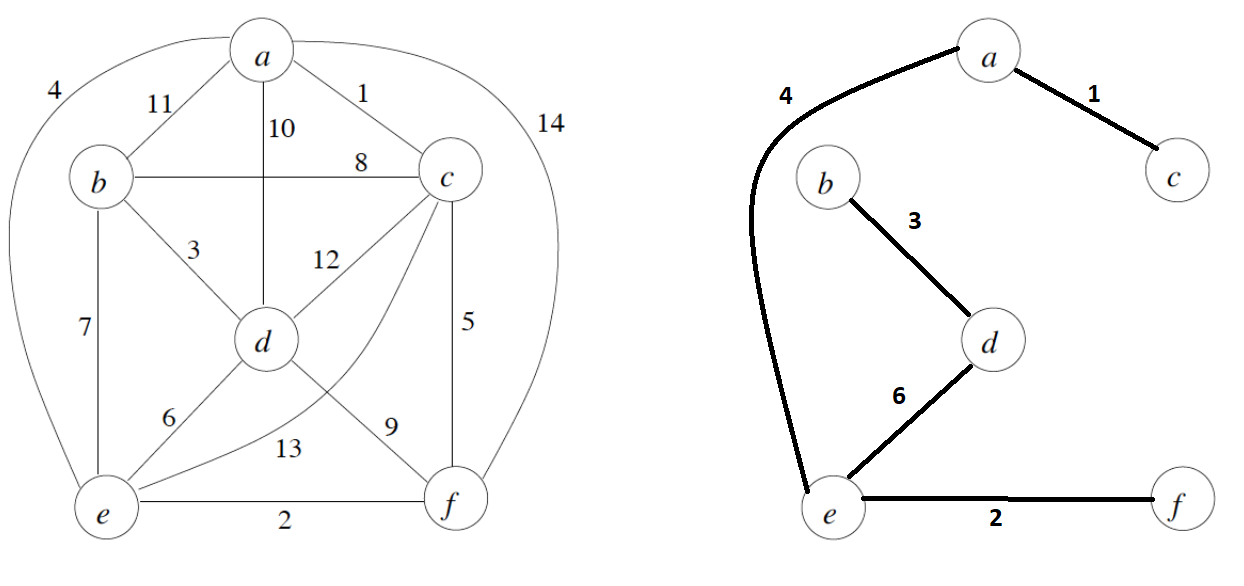
\includegraphics[width=\textwidth]{1a}
\end{center}
\end{figure}

(b) Fill out the table below with the edges of the above minimum spanning tree according to their orders of selection by Kruskal's 
and Prim's algorithms, respectively.

\begin{figure}[htb]
\begin{center}
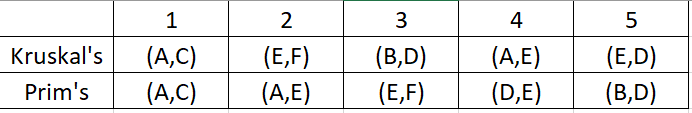
\includegraphics[width=\textwidth]{1b}
\end{center}
\end{figure}

(c) Suppose all edges in a graph $G$ have different edge weights. Show that $G$ has a unique minimum spanning tree. 
\smallskip
\\
We have G=(V,E) defined as the graph, with this set...\\
Supposed there are two different minimum spanning trees (MST), $T_1$ and $T_2$. they have the sets pf $E_1$ and $E_2$, and when subtracted as such: 
\\$E_1 - E_2$ and then as $E_2 - E_1$, they are not empty. thus we can come to the conclusion that $\exists e \epsilon  E_1 - E_2$. Due to the nature of $e \epsilon E_2$ when being added to $T_2$, we can identify it as a cycle and thus apply the cycle property. This property states that the most expensive edge (e') does not belong to any MST.\\
if e' = e then e' $\epsilon E_1$ because of $e \epsilon E_1 - E_2$\\
else if e' $\neq$ e then e' $\epsilon E_2$
\newpage
\hrulefill \\


\textbf{Problem 2:} (Shortest Paths)\hfill (20 Points)\\

(a) Consider the graph $G$ below.
\begin{figure}[htb]
\begin{center}
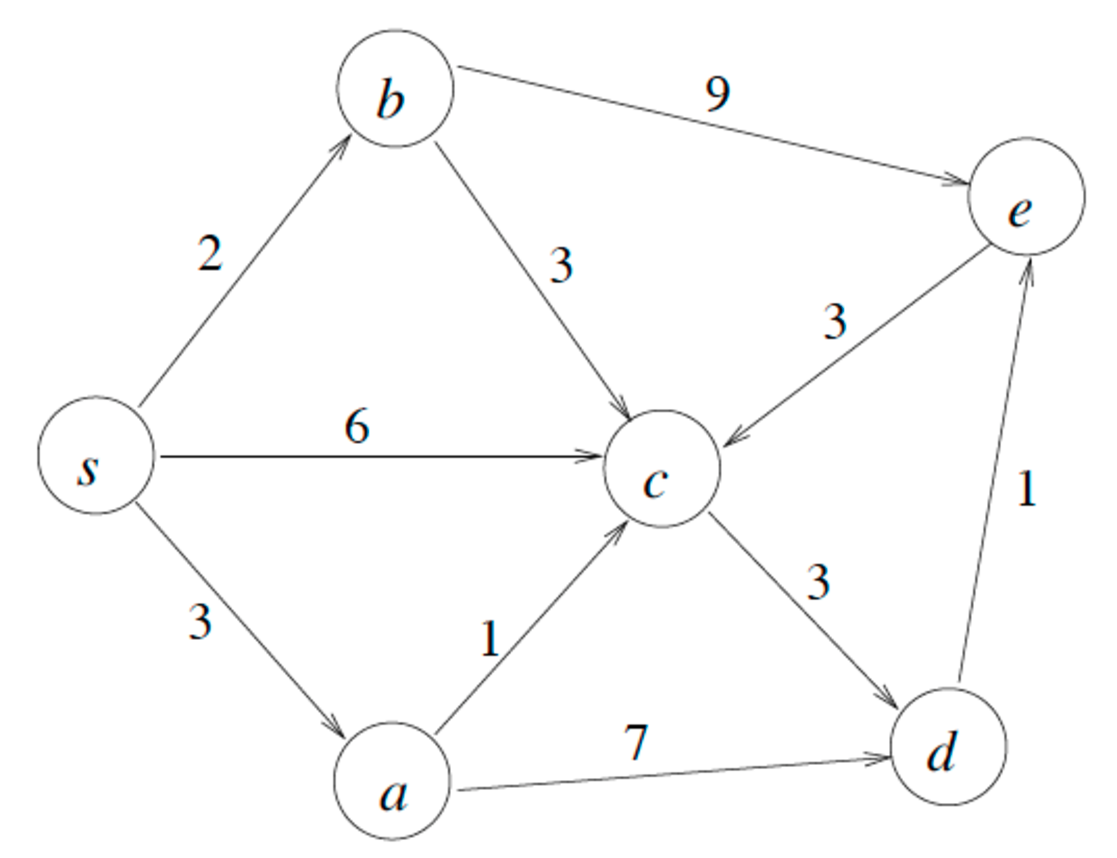
\includegraphics[width=6cm]{SP}
\end{center}
\end{figure}

Show the execution of Dijkstra's algorithm on $G$ by filling out the table below. Assume the source is vertex $s$. You must show the changes in the
d-array at the end of each iteration. Iteration 0 refers to the situation just before the first  iteration of the {\bf while} loop. Also, fill in the vertex that is selected (i.e., extracted from the priority queue) at each iteration.
\begin{figure}[htb]
\begin{center}
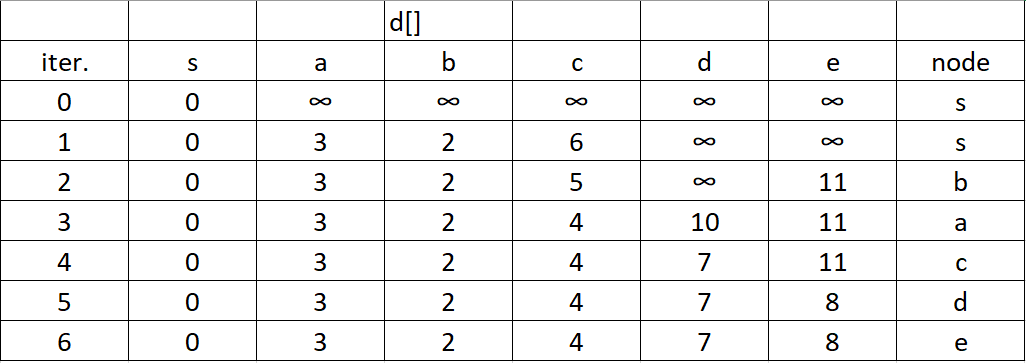
\includegraphics[width=11cm]{2a}
\end{center}
\end{figure}

\newpage
\hrulefill \\

(b) Draw a shortest path tree for the graph in (a) with source vertex $s$.
\begin{figure}[htb]
\begin{center}
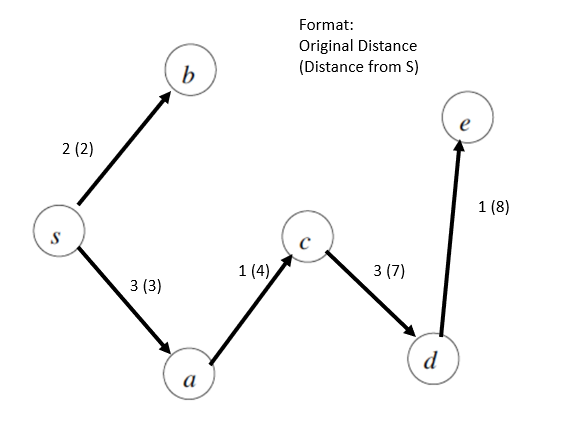
\includegraphics[width=11cm]{2b}
\end{center}
\end{figure}
\newpage
\hrulefill \\

(c) Suppose that all edge weights in a given graph $G:=(V,E)$ are NOT negative, and that the shortest path distances in $G$ from a source $s\in V$ to each vertex $v\in V$ are unique. Let $V_k$ denote the vertices in $V$ with the $k$-closest shortest path distances from $s$.\\

\underline{Example:} Let $V=\{s, u, v\}$ and $0, 2, 3$ be the shortest path distances of the vertices  $s, u, v$ from $s$ in $G$ respectively. Then, $s$ is the $1$-closest vertex, $u$ is the $2$-closest vertex, and $v$ is the $3$-closest vertex. Therefore we have $V_1= \{s\}$, $V_2=\{s,u\}$, $V_3=V$.\\ 

Prove by contradiction that a shortest path from the source vertex $s\in V$ to a k-closest vertex $x\in V$ consists only of vertices in $V_k$. 
\\\\
Proof via contradiction:\\
There is some vertex not in V (the shortest path), $v \notin V$. There exists another path including said $v$. The path will continue with the path going through vertex $v$ until reaching the destination $V_k$, however once it arrives at such, we can identify the issue; as we have introduced excess length/weight into the path. We have now visited a vertex that was not in the original list of verticies. Due to this, when we try to get to a vertex $V_k$, but eventually there will be a point where $V_n$ will differ from what the expected value of $V_n$ should be due to the introduction of a $v \notin V$ This occurs because the path in the orignal V is distinct. 
\newpage
\hrulefill \\
\textbf{Problem 3:} (P is Closed under Reverse Complement)\hfill (20 Points)\\

Consider the operation of reverse complement on a language over the alphabet $\{ 0, 1\}$. The reverse complement of a string $x \in \{ 0, 1 \}^*$ of length $n$ is a string $y \in \{ 0, 1 \}^*$ of the same length such that $y_k = 1 - x_{n-k+1}$ for $k = 1, 2, ..., n$, where $y_k$ is the bit at index $k$ of string $y$. Let $\overline{x}$ denote the reverse complement of string $x$. For example, if $x = 011101$, then $\overline{x} = 010001$. Note that $\overline{x}$ is obtained from  $x$ by reversing its bit sequence
and complementing each bit (changing $1$ to $0$ and $0$ to $1$). Let $L$ be a language over the alphabet $\{ 0, 1\}$. The reverse complement of $L$ is defined as \\

$\overline{L} = \{ \overline{x} : x \in L \}$. \\

Show that if $L$ is in P, then $\overline{L}$ is also in P. Note that the reverse complement of $L$ is not related to the set complement of $L$. Your algorithm takes as input a binary string in $\{ 0, 1 \}^*$.
\begin{algorithm}[H]
    \Fn(){bitShit()}{
    \KwIn{Binary String $str$}
    \SetAlgoLined
    \SetNoFillComment
    BinaryString y\\
    for(i = 0 to str.size)\\
        \hspace{.5cm}y[i] = 1 - x[str.size - i + 1]\\
    return y\\
    }
\end{algorithm}
\smallskip
This algorithm goes through the entireity of X and places the last element within x into the first slot of y and walks down y and up x at the same time to both switch the places of the bits in the string and also inverts the bit. The runtime of this algorithm goes to $O(N)$ due to the loop, it iterates through the entireity of X. The verifier of this algorithim has to run in polynomial time for this to return true, and since it does, this algorithim also does so.
\newpage
\hrulefill \\
\textbf{Problem 4:} (String Transformation is in NP)\hfill (20 Points)\\

A string $x \in \{ 0, 1 \}^*$ is transformed into another string $y$ by a sequence of operations of two types. Let $x$ be a string of $n$ bits, indexed from $1$ to $n$, where $x_{i,j}$ denotes a substring of $x$, consisting of consecutive bits from index $i$ to index $j$ in the same order, with $1 \leq i \leq j \leq n$. Let $xyz$ denote the concatenation of strings $x$, $y$, and $z$. An inversion operation $r(i,j)$ turns string $x$ into $x_{1, i-1} \overline{x_{i, j}} x_{j+1, n}$, with $1 \leq i \leq j \leq n$, where $\overline{x_{i, j}}$ is the reverse complement of $x_{i, j}$ (see problem 3). A deletion operation $d(i,j)$ turns string $x$ into $x_{1, i-1} x_{j+1, n}$. For example, an inversion operation $r(3, 6)$ transforms string $11011100$ into string $11000100$ ($x_{3, 6} = 0111$, $\overline{x_{3, 6}} = 0001$), which is further transformed into string $100100$ by a deletion operation $d(2, 3)$.
Show that the problem of deciding whether a string can be
transformed into another string by a sequence of at most $k$ operations of
substring deletions and inversions is in NP. Specifically, the problem is defined
as the formal language \\

$\textrm{ST} = \{ <x, y, k>: \textrm{there exists a sequence of at most}\; k \; \textrm{operations}$

$\qquad \qquad \textrm{of deletions and inversions to transform binary strings}\; x\; \textrm{into}\; y\; \}$. \\

Show that ST is in NP. Note that your algorithm takes two types of input: one type is an ordinary input including two strings $x$ and $y$ along with an integer $k$, and the other is a certificate.
\\\\
In order for ST to be in NP (a set of languages) there needs to be an efficent polynomial time certifier that can effectively run a specific instance with the correct certificate. If we can determine x and y in polynomial time via a correct certificate, it will be in NP time as a whole. The method below verfies that strings X and Y via the following:\\L $= \{ x \in \{0,1\}^*, y \in \{0,1\}^*, k:$ there exists a certificate, $cert \in \{0,1\}^*$, with $|cert| = O(|x|^c)$\\ We can determine the algorithim verifies language L in polynomial time which means when we have the right certificate it was decided in P time making the language ST in NP. This was completed within K total operations\\
%The instance input is string x, y, and int k, and also the certificate is an input. such that stringTransformNP(x,y,k,certy) $= 1 \}$\\
\begin{algorithm}[H]
    \Fn(){stringTransformation()}{
    \KwIn{String x, String y, int k, Certificate cert}
    \SetAlgoLined
    \SetNoFillComment
    if(x == y) //end condition\\
        \hspace{.5cm}return true\\
    if(k $\geq$ actionsRemaining) //checks if theres enough actions left against a global var\\
        \hspace{.5cm}if(x $>$ cert.size)\\
            \hspace{1cm}for i to size of x\\
                \hspace{1.5cm}for j to size of x\\
                    \hspace{2cm}if(deletion(i, j) == cert)\\
                        \hspace{2.5cm}return true\\
        \hspace{.5cm}else if(x $<$ cert.size)\\
            \hspace{1cm}for i to size of x\\
                \hspace{1.5cm}for j to size of x\\
                    \hspace{2cm}if(revise(i, j) == cert)\\
                        \hspace{2.5cm}return true\\
        \hspace{.5cm}return false\\
    }
\end{algorithm}

\newpage
\hrulefill \\
\textbf{Problem 5:} (Restricted CNF-SAT is in P)\hfill (20 Points)\\

A boolean formula in conjunctive normal form, or CNF, is expressed as an AND of clauses, each of which is the OR of one or more literals. A restricted CNF formula meets the following requirements. For every clause with two or more literals in the formula, if the clause contain literal $x$, then no clause can contain $\neg x$, and if it contain $\neg x$, then no clause can contain $x$. If any clause with only one literal contains $x$ or $\neg x$, then this literal cannot occur in any clause with two or more literals. For example, the boolean formulas, \\

$(x_1 \vee \neg x_2 ) \wedge (\neg x_3 \vee x_4 \vee x_5 ) \wedge x_6 \wedge \neg x_6$, and

$(x_1 \vee \neg x_2 ) \wedge (\neg x_3 \vee x_4 \vee x_5 ) \wedge x_6 \wedge \neg x_7$, \\

meet the requirements, and the following formulas do not, \\

$(x_1 \vee \neg x_2 ) \wedge (\neg x_3 \vee x_4 \vee x_5 ) \wedge x_2$, and

$(x_1 \vee \neg x_2 ) \wedge (\neg x_1 \vee x_2 \vee x_5 )$. \\

Show that the problem of deciding whether a restricted boolean formula in CNF is satisfiable is in P. Specifically, the problem is defined as the formal language \\

$\textrm{RES-CNF} = \{ <\theta> : \theta \; \textrm{is a satisfiable restricted boolean formula in CNF} \}$. \\

Show that RES-CNF is in P. Note that input to your algorithm is a restricted boolean formula in CNF.
\smallskip\\
\begin{algorithm}[H]
    \Fn(){restrictedCNF()}{
    \KwIn{Array of CNF formula, $input$}
    \SetAlgoLined
    \SetNoFillComment
    \DontPrintSemicolon
    for($i = 0$ to $input.length$) //runs through the length of input once here\\
        \hspace{.5cm}if((input[i]+1 == $\bigwedge $ AND i == 0) OR (input[i]-1 == $\bigwedge $ AND i == input.size-1))\\
            \hspace{1cm}add to single literal list //constant time\\
            
        \hspace{.5cm}else if(input[i]+1 == $\bigwedge $ AND input[i]-1 == $\bigwedge $)\\
            \hspace{1cm}add to single literal list //constant time\\
    for($i = 0$ in literalList.size) //run through length of input\\
        \hspace{.5cm}for($j=0$ in literalList.size) //run through length of input again with j instead of i\\
            \hspace{1cm}if(input[i] == input[j].not)\\
                \hspace{1.5cm}return false\\
    return true
    }
    \end{algorithm}
    \smallskip
    The definition of polynomial time is if something is $O(n^k)$, and the algorithm given above has a run time of $O(n+n^2)$ which runs to $O(n^2)$ which is a polynomial time. By reading the restricted boolean CNF input, we determine where we are currently checking in the first for loop, if the element is surrounded by nothing else but $\bigwedge$ then it is added to the list, but we also have to check if the element is the first or last element in the listing, as nothing would be surronding it, so we check those edge cases as well. 
    
\end{document}